\chapter{Methodology}
\label{ch:methods}

\section{System Architecture}

The proposed pipeline, illustrated in Figure~\ref{fig:system_overview}, consists
of three major stages executed sequentially on each code commit:

\begin{enumerate}
  \item \textbf{Static Analysis --- CodeQL SAST.} CodeQL is executed against each
        commit to generate a SARIF-format alert report. SARIF (Static Analysis
        Results Interchange Format) is a vendor-neutral JSON schema that captures
        per-alert information including file path, line number, rule identifier,
        message, and severity.
  \item \textbf{Feature Extraction and ML Classification.} SARIF results are
        parsed; contextual code features are extracted from source files; and
        machine learning classifiers assign each alert a confidence score
        indicating the probability that it is a true vulnerability.
  \item \textbf{Agentic Triage and Remediation.} Alerts above a confidence
        threshold are passed to the agentic AI layer, which evaluates vulnerability
        type, generates contextual remediation suggestions, and outputs actionable
        findings including automated code patches.
\end{enumerate}

\begin{figure}[htbp]
  \centering
  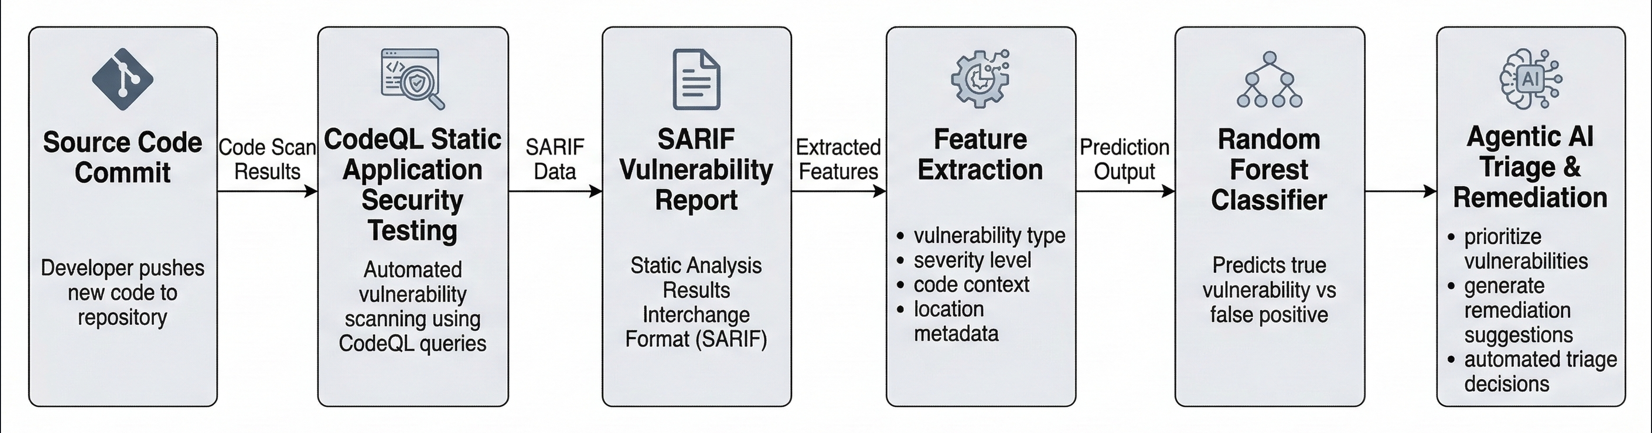
\includegraphics[width=\textwidth]{Figures/fig_system_overview.png}
  \caption{Agentic AI pipeline for automated vulnerability detection and triage.
           The pipeline transforms raw source code into prioritised, actionable
           vulnerabilities with confidence scores and remediation suggestions.}
  \label{fig:system_overview}
\end{figure}

\section{Dataset: OWASP Benchmark}

The OWASP Benchmark Project provides 2,766 Java test cases covering eight
vulnerability categories: SQL Injection (Sqli), OS Command Injection (Cmdi),
XSS (Cross-Site Scripting), Path Traversal, Insecure Randomness, Cryptographic
Weakness, LDAP Injection, and Weak Hashing. Each test case has a binary ground
truth label. The dataset is specifically designed for SAST evaluation and is
widely used in the research community.

\section{Feature Extraction from SARIF}

\begin{figure}[htbp]
  \centering
  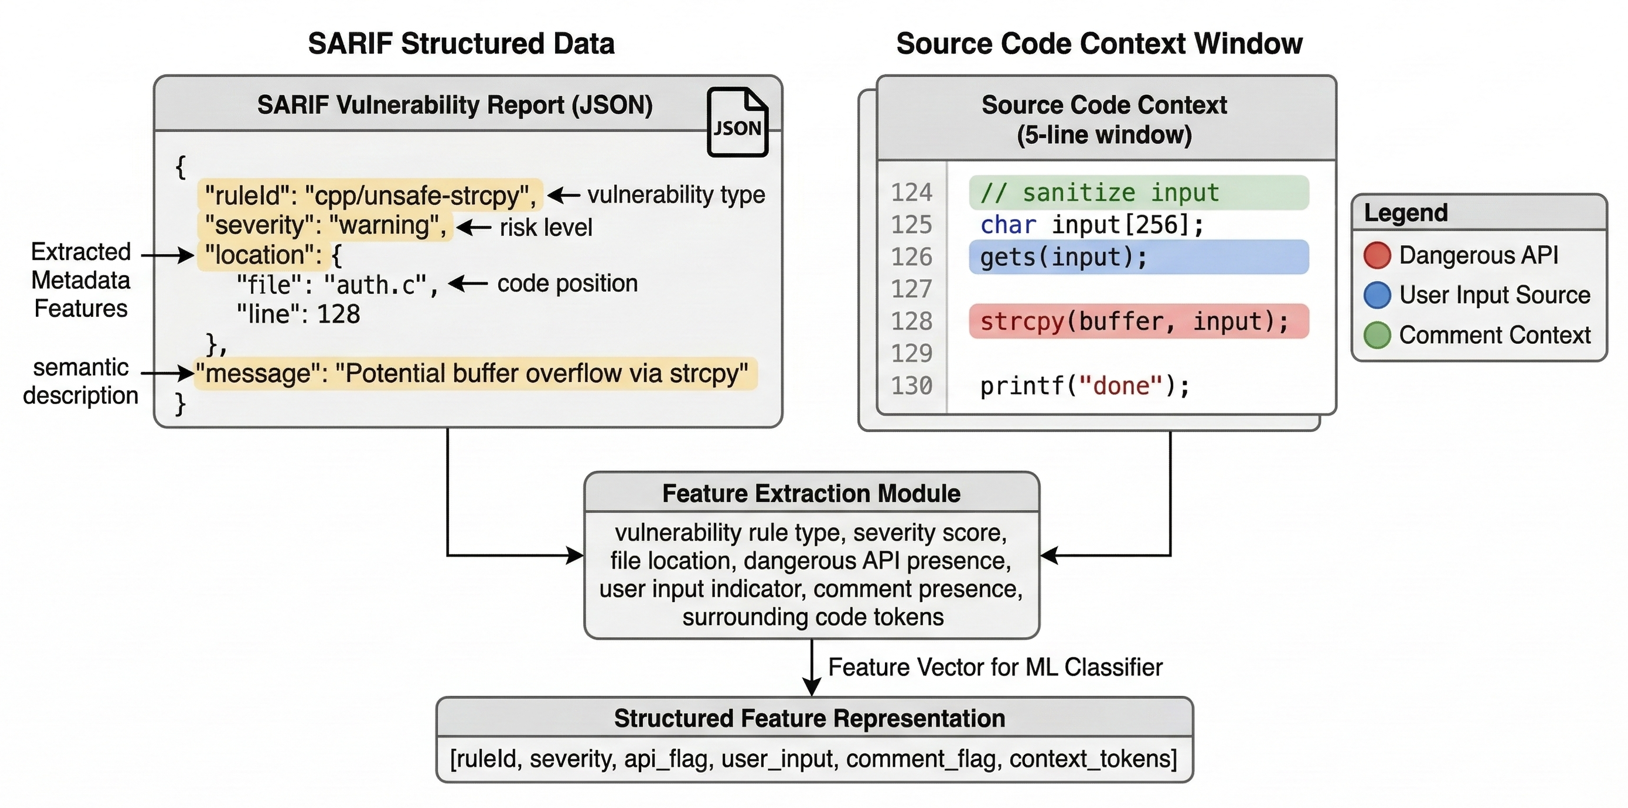
\includegraphics[width=\textwidth]{Figures/fig_feature_extraction.png}
  \caption{Feature extraction process. SARIF metadata provides basic features;
           source code context around the alert line provides contextual features
           for the ML classifiers.}
  \label{fig:feature_extraction}
\end{figure}

CodeQL SARIF output provides per-alert metadata. As shown in Figure~\ref{fig:feature_extraction},
we construct the following feature set for each alert. The feature set evolved significantly over the
course of the project from basic SARIF metadata features to a richer, vectorized representation.

\subsection{Basic Features (Iteration 1)}

The initial feature set used only raw SARIF metadata:
\begin{itemize}
    \item \textbf{Rule identifier (CWE)} --- Categorical, from SARIF
    \item \textbf{Severity level} --- Ordinal, from SARIF
    \item \textbf{Alert location (line)} --- Numeric, from SARIF
    \item \textbf{File alert density} --- Numeric, from SARIF
    \item \textbf{Dangerous API present} --- Binary, from source code
    \item \textbf{User input source} --- Binary, from source code
    \item \textbf{Surrounding comment} --- Binary, from source code
\end{itemize}

\subsection{Vectorized Feature Representation (Final)}

The final, improved feature set transitioned from a single \texttt{alert\_count} feature
to a 13-dimension vectorized representation of vulnerability types, coupled with weighted
feature engineering. The key additions are:

\begin{table}[htbp]
  \centering
  \caption{Final Feature Set for ML Classifiers (Vectorized)}
  \label{tab:features}
  \renewcommand{\arraystretch}{1.2}
  \begin{tabular}{p{5cm}ll}
    \toprule
    \textbf{Feature} & \textbf{Type} & \textbf{Source} \\
    \midrule
    Rule identifier (CWE) one-hot & Categorical/Vector & SARIF \\
    Severity level & Ordinal & SARIF \\
    Alert location (line) & Numeric & SARIF \\
    File alert density & Numeric & SARIF \\
    \texttt{same\_type\_count} & Numeric & Derived \\
    \texttt{weighted\_alert\_count} & Numeric & Derived \\
    Dangerous API present & Binary & Source \\
    User input source & Binary & Source \\
    Surrounding comment & Binary & Source \\
    \bottomrule
  \end{tabular}
\end{table}

The \texttt{same\_type\_count} feature counts how many alerts of the same CWE type appear
in the same file. The \texttt{weighted\_alert\_count} applies category-specific weights
to give higher importance to historically more impactful vulnerability types (e.g., SQL
Injection, Command Injection). The one-hot encoded rule identifier expands to a
13-dimension vulnerability type vector rather than a single aggregate count, giving the
classifier much greater discriminative power.

\section{Machine Learning Models}

Three classifiers were trained and compared:

\begin{enumerate}
    \item \textbf{Random Forest (RF):} A parallel bagging ensemble of 200 decision trees with
          \texttt{class\_weight=`balanced'} and \texttt{n\_jobs=-1} for parallel training.
          Handles non-linear relationships and is robust to noisy features.
    \item \textbf{Gradient Boosting (GBM):} A sequential boosting ensemble with 200 estimators,
          learning rate 0.08, max depth 4, subsample 0.8. Minimizes loss iteratively and
          captures complex feature interactions.
    \item \textbf{Support Vector Machine (SVM, RBF kernel):} Wrapped in a scaling pipeline.
          An RBF-kernel margin-based classifier with \texttt{C=5.0}, \texttt{gamma=`scale'},
          and balanced class weights.
\end{enumerate}

All models used a stratified 70/30 train/test split. The \texttt{ml\_dataset\_weighted.csv}
dataset (4,138 samples: 2,703 vulnerable, 1,435 non-vulnerable) was used for all comparisons.

\section{Threshold Optimization}

A key methodological contribution is the identification of the optimal decision threshold
per model. Instead of using the default 0.5 threshold, we computed accuracy at 200 evenly
spaced threshold points from 0.01 to 0.99 and selected the argmax:

\[
  t^* = \arg\max_{t \in [0,1]} \; \text{Accuracy}(y, \hat{y}_t)
\]

where $\hat{y}_t = \mathbf{1}[\hat{p} \geq t]$ and $\hat{p}$ is the predicted class
probability from the model.

\section{Agentic Triage and Remediation}

\begin{figure}[htbp]
  \centering
  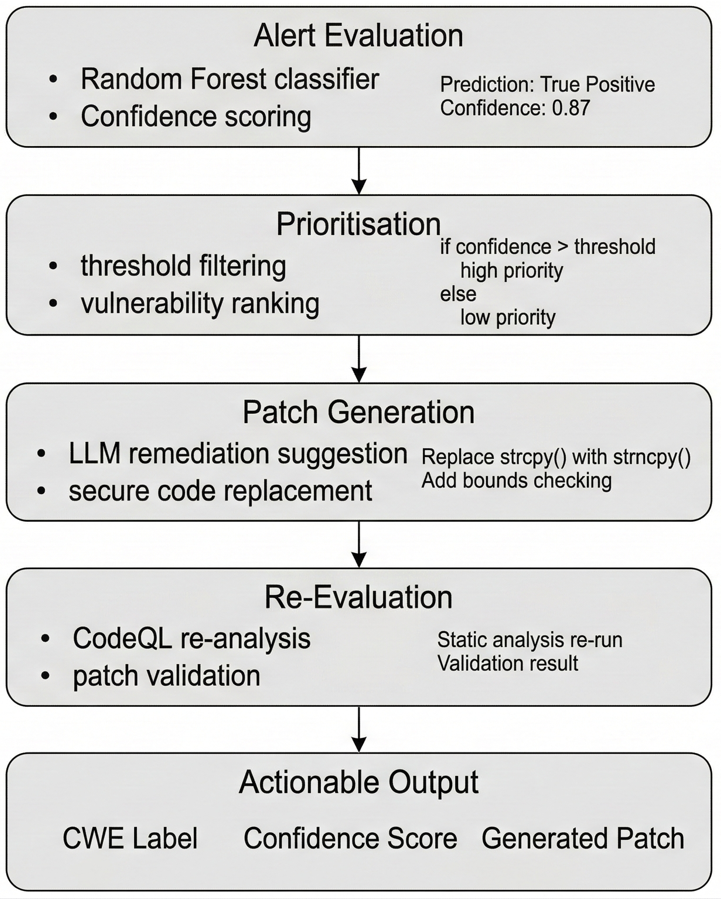
\includegraphics[width=0.85\textwidth]{Figures/fig_agentic_triage.png}
  \caption{Agentic triage and remediation workflow. The agentic layer converts
           classifier output into developer-actionable patches.}
  \label{fig:agentic_triage}
\end{figure}

High-confidence alerts from the classifier are passed to the agentic AI layer
(Figure~\ref{fig:agentic_triage}). The workflow:

\begin{enumerate}
  \item \textbf{Alert Evaluation.} The ML model classifies each alert and assigns a
        confidence value.
  \item \textbf{Vulnerability Prioritisation.} Alerts above the optimized confidence
        threshold ($t^*$) are marked as actionable vulnerabilities.
  \item \textbf{Patch Generation.} For confirmed vulnerabilities, an LLM generates a
        remediation suggestion based on the vulnerability type (CWE category) and the
        surrounding code context.
  \item \textbf{Patch Application and Re-Evaluation.} The patched code is re-analysed
        using CodeQL to verify that the vulnerability is resolved and no new issues are introduced.
\end{enumerate}